\section{Task 2: Model Adaptation and Migration}

In the previous section, we have established a model to quantify 
the tourism industry in Juneau. 
Based on this model we take a further look at the city of Sitka, Alaska and
test the model's adaptability and migration capability.

The following analyses, calculations and predictions are identical to those done
in the area of Juneau. The model is adapted to the city of Sitka, and the optimal tax rate, number of tourists, and fine rate are calculated.

\subsection{Procedure}

We first calculated the CG of Sitka, Alaska, and utilized the results
to predict the ratio of tourists to local residents in the next few years.
The CG prediction is shown in subplot 2. After that, we extrapolate the relationship
between CG and the number of tourists, and forcast GDP in the next few years.
After that, according to equation (8), we forcast the amount of carbon emission
from tourism in the next few years. The results are shown in subplot 5. In addition, 
we assume that the price of carbon increases by 5\% each year, carbon price prediction 
can thus be obtained. The results are shown in subplot 4. Finally, we use the equation
$\text{Carbon Cost} = \text{Carbon Emission} \times \text{Carbon Price}$ to calculate the
carbon cost in the next few years. The results are shown in subplot 7 and 8.

\subsection{Results}

The results of the prediction are shown in the following table.

\begin{figure}[H]
    \centering
    \begin{minipage}[t]{0.32\textwidth}
        \centering
        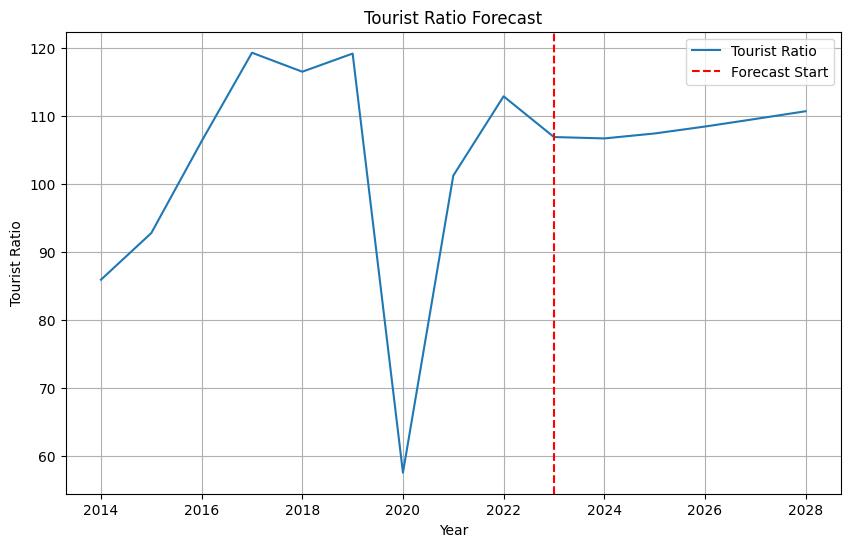
\includegraphics[width=1\textwidth]{Ratio_Sitka.png}
    \end{minipage}
    \hfill
    \begin{minipage}[t]{0.32\textwidth}
        \centering
        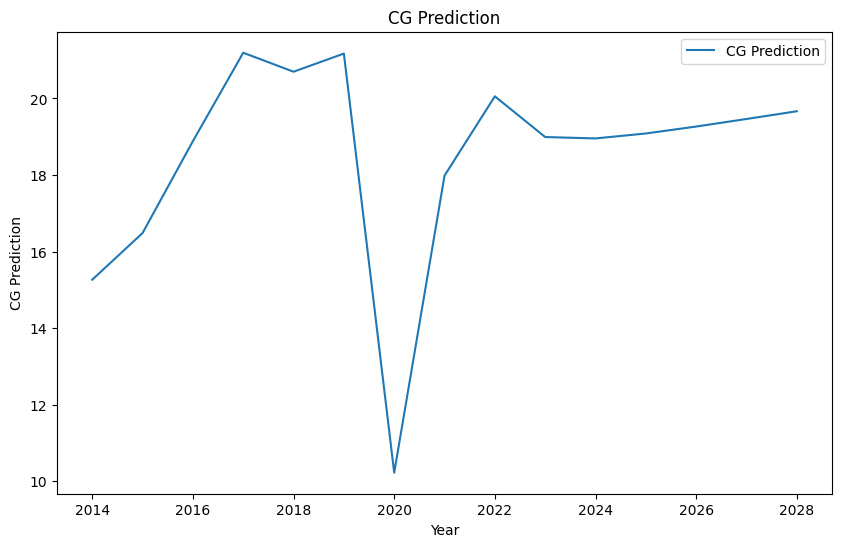
\includegraphics[width=1\textwidth]{CG_Sitka.png}
    \end{minipage}
    \hfill
    \begin{minipage}[t]{0.32\textwidth}
        \centering
        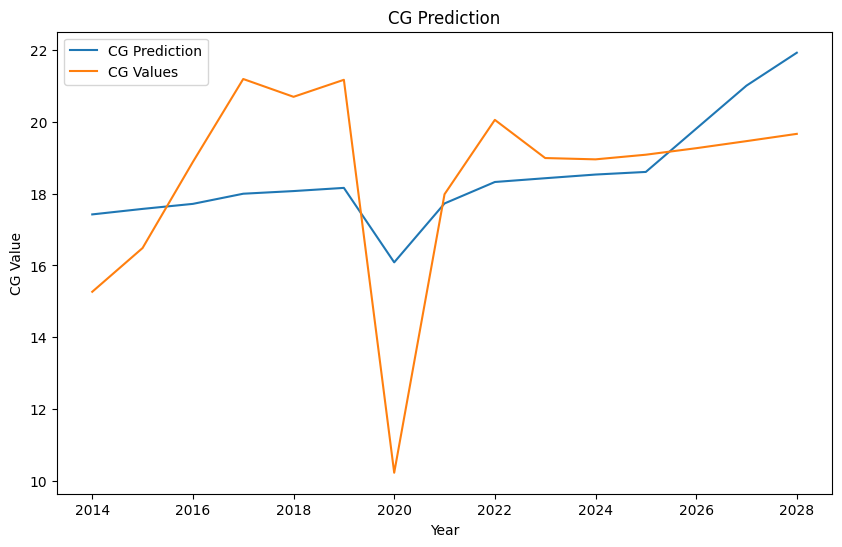
\includegraphics[width=1\textwidth]{CG_Pred_Sitka.png}
    \end{minipage}
\end{figure}

\begin{figure}[H]
    \centering
    \begin{minipage}[t]{0.32\textwidth}
        \centering
        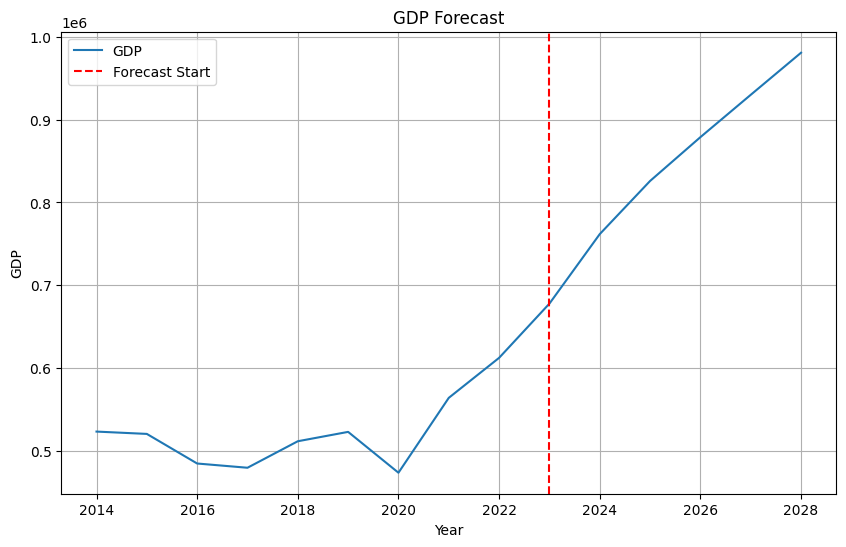
\includegraphics[width=1\textwidth]{GDP_Sitka.png}
    \end{minipage}
    \hfill
    \begin{minipage}[t]{0.32\textwidth}
        \centering
        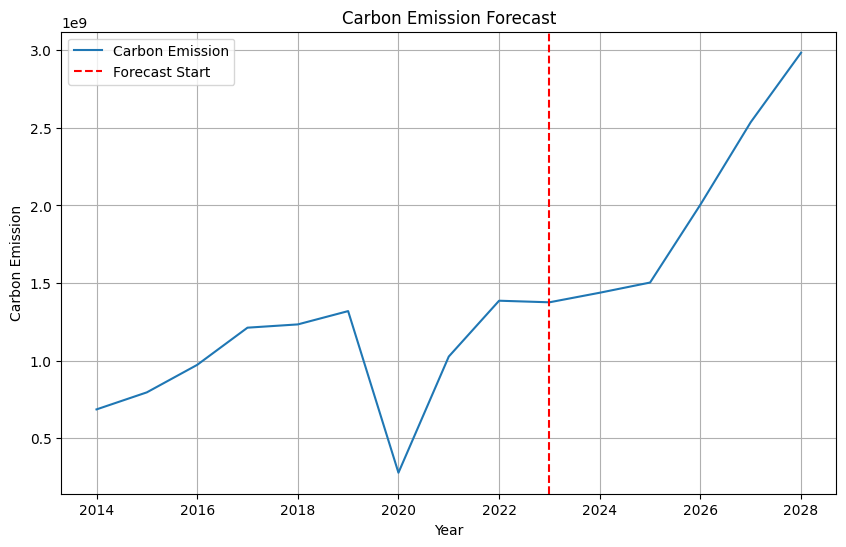
\includegraphics[width=1\textwidth]{C_Emission_Sitka.png}
    \end{minipage}
    \hfill
    \begin{minipage}[t]{0.32\textwidth}
        \centering
        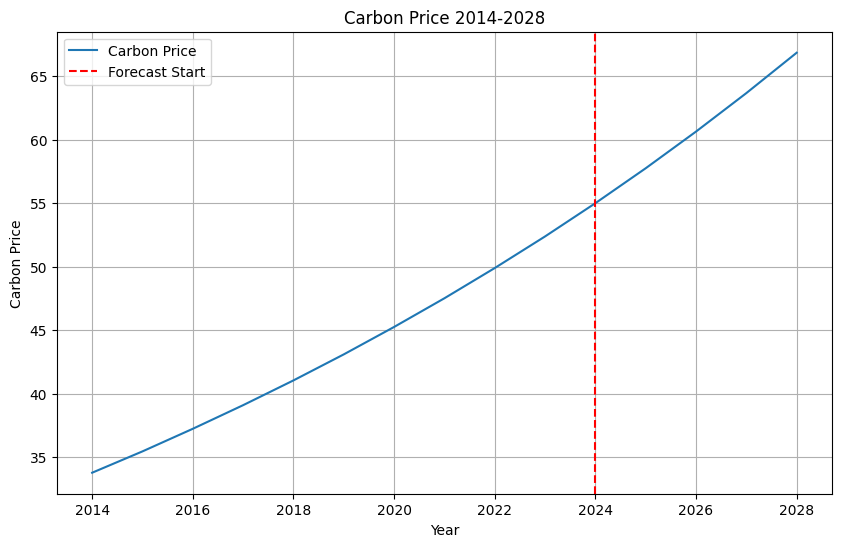
\includegraphics[width=1\textwidth]{C_Price_Sitka.png}
    \end{minipage}
\end{figure}

\begin{figure}[H]
    \centering
    \begin{minipage}[t]{0.49\textwidth}
        \centering
        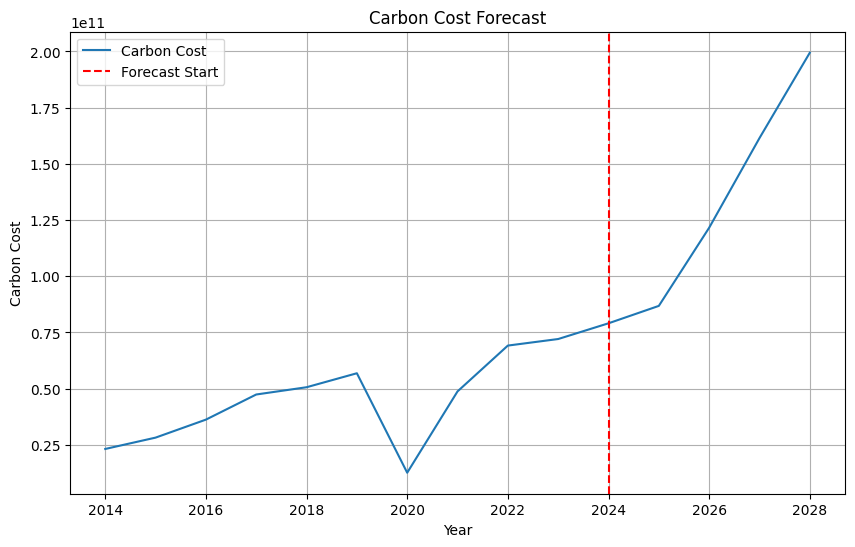
\includegraphics[width=1\textwidth]{C_Cost_Sitka.png}
    \end{minipage}
    \hfill
    \begin{minipage}[t]{0.49\textwidth}
        \centering
        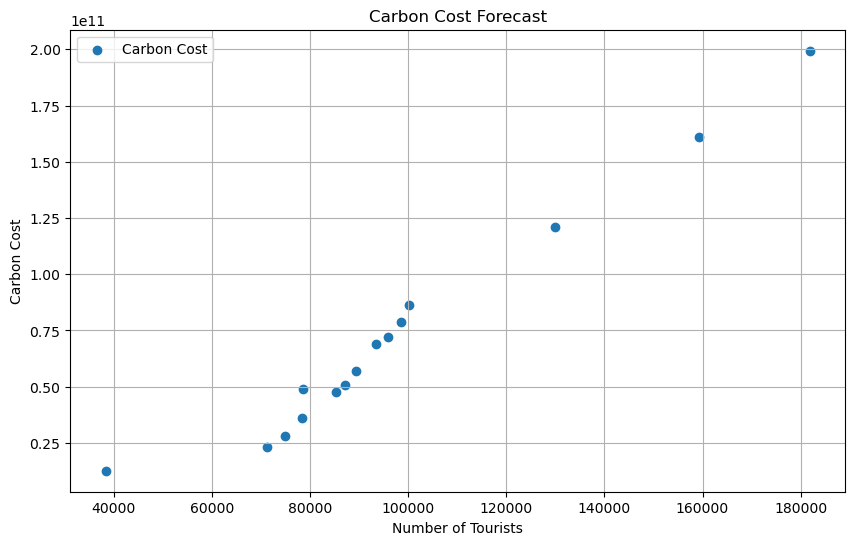
\includegraphics[width=1\textwidth]{C_to_People_Sitka.png}
    \end{minipage}
\end{figure}

\subsection{Analyses}

Summing up all the categories and the parameters yields the final equation.

\begin{equation}
    \begin{aligned}
    &\left\{\begin{array}{l}
    \mathcal{F}=(\alpha \cdot \text { Economy }-\beta \cdot \text { Environment }) / \text { Society } \\[10pt]
    \text { Economy }=165 N \cdot f(\eta) \cdot (\eta+1)+NQ\cdot e^{-0.2 Q} \\[10pt]
    \text { Environment }=2.897 \cdot N^2+ 7.67\times 10^5 N- 3.293\times 10^{10} \\[10pt]
    \text { Society }=5.011\times 10^{-9} N + 4.2 \\[10pt]
    f(\eta)=-5.5 \eta^3+9.1903 \eta^2-5.1903 \eta+1.5, \quad 0 \leq \eta \leq 1
    \end{array}\right.
    \end{aligned}
\end{equation}

When $\alpha$ is set to 1 and $\beta$ is set to 30, 
the optimal value of $N,Q,\eta$ is calculated as follows:

\begin{equation}
    \begin{aligned}
    &\left\{\begin{array}{l}
    N_{Max} = 93.353 \\[10pt]
    N_{LastYear} = 95.937 \\[10pt]
    N=52.04 \\[10pt]
    Q=4.89 \\[10pt]
    \eta=0.286
    \end{array}\right.
    \end{aligned}
\end{equation}

The strategy is the same as we have proposed in Juneau, 
that is to increase the tax rate and the fine rate, and to 
decrease the number of tourists. Thus our model can be successfully
adapted to Sitka, Alaska, proving its adaptability and migration capability.

\subsection{Sensitivity Analysis}

To evaluate the robustness of the migrated model, we conduct a sensitivity analysis.

The results are shown below:

\begin{figure}[H]
    \centering
    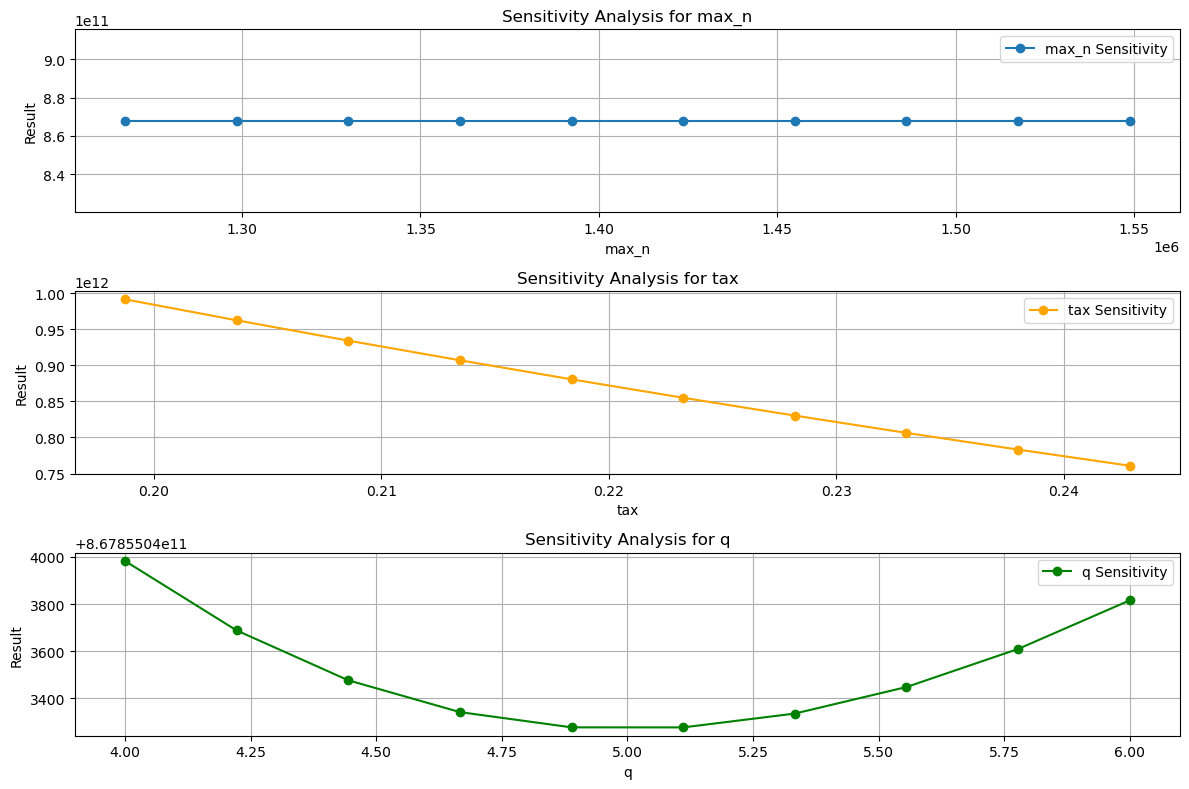
\includegraphics[width=1\textwidth]{Sensitivity_Analysis_Sitka.jpg} % 插入图片
    \vspace{-0.5cm}
    \caption{Sensitivity Analysis}
\end{figure}

It can be shown that when $N_{Max}$ is the independent variable, the outcome is immune to the change of $N_{Max}$,
while in other circumstances are sensitive to the changing of the independent variables.
The result is similar to what we conducted in Juneau.